\scanpage{13}
% Reader A; one-page independent reading. Coordinates in the figure use the full scan.
% No compiler or renderer used; graphical paths are direct approximations of inspected ink.
% Upper left marginal cluster; its internal positions follow the original pixels.
\margin{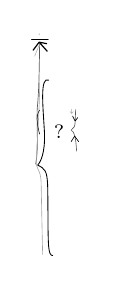
\begin{tikzpicture}[x=.00635cm,y=-.00635cm,line cap=round,line join=round]
\path[use as bounding box] (24,391) rectangle (145,861);
% M01: bar and upward shaft, with separately visible retracing.
\draw[line width=.42pt] (32,414)--(65,414);
\draw[black!65,line width=.25pt] (48,422)..controls (47,477) and (47,514)..(43,554)..controls (42,597) and (46,631)..(40,664);
\draw[line width=.43pt] (35,436)--(47,420)--(63,438) (47,420)--(62,423);
\draw[black!35,line width=.18pt] (47,426)--(38,448);
% M02: long brace, and pale independently visible parallel continuation.
\draw[line width=.31pt] (66,496)..controls (48,487) and (55,553)..(57,591)..controls (60,629) and (54,655)..(44,666)..controls (58,673) and (63,676)..(64,708)..controls (65,755) and (64,805)..(66,829)..controls (67,842) and (70,847)..(74,847);
\draw[black!35,line width=.22pt] (48,500)..controls (48,552) and (43,612)..(41,663)..controls (44,678) and (51,678)..(51,705)..controls (52,753) and (53,809)..(54,845);
\draw[line width=.18pt] (48,556)..controls (40,565) and (43,586)..(48,604);
% M03: question mark and opposed arrows, including the intervening curved stroke.
\node[font=\scriptsize] at (87,600) {?};
\draw[black!65,line width=.23pt] (120,555)--(119,578)..controls (119,588) and (117,592)..(111,596)..controls (118,600) and (120,610)..(122,638);
\draw[line width=.24pt] (114,568)--(119,578)--(124,571) (111,619)--(118,608)--(126,619);
\draw[black!32,line width=.17pt] (112,554)--(112,563) (109,559)--(112,563)--(115,559);
% M04: detached small grey mark above the bar; role and hand undetermined.
\fill[black!40] (47,404) ellipse[x radius=.9,y radius=1.8];
\end{tikzpicture}}
\figure{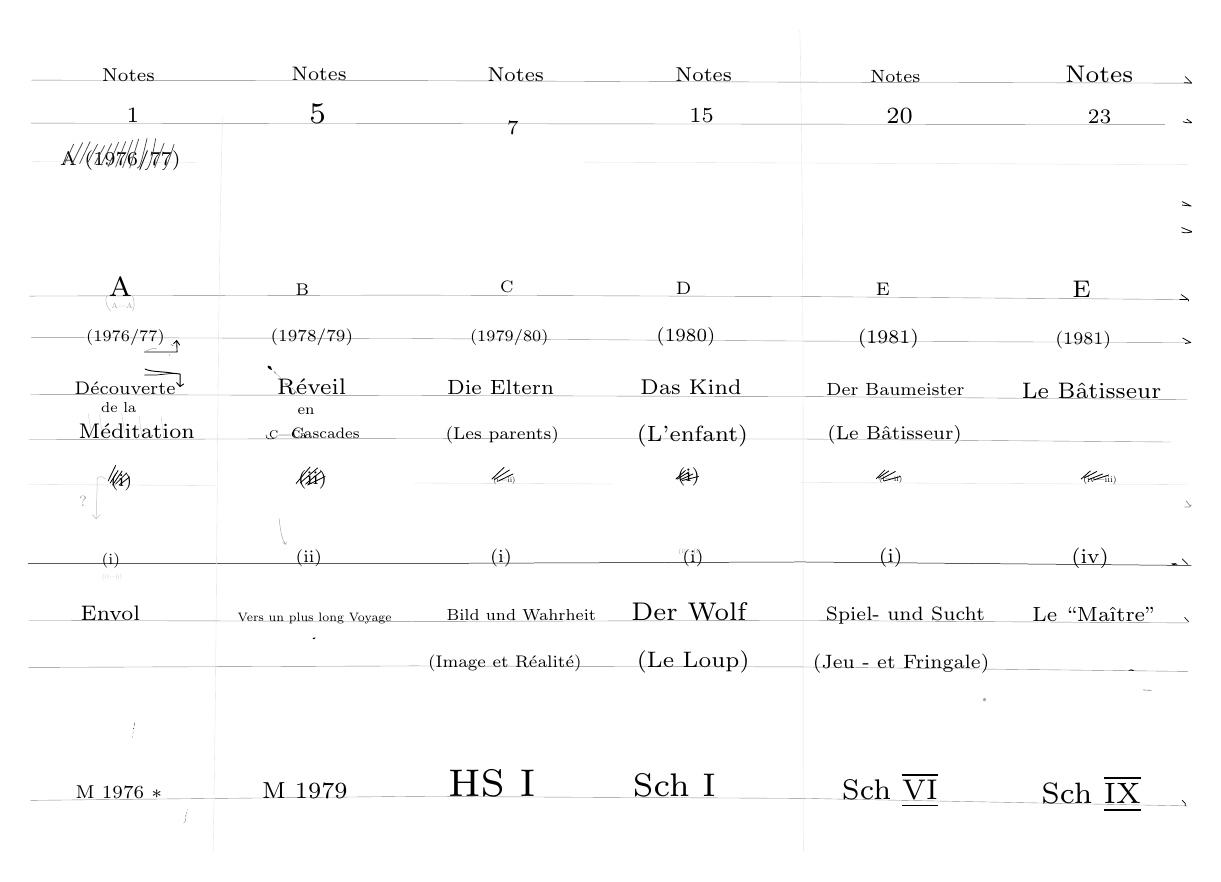
\begin{tikzpicture}[x=.00635cm,y=-.00635cm,line cap=round,line join=round]
\path[use as bounding box] (20,18) rectangle (2352,1670);
% R01--R12: visible horizontal rules; no extrapolated equal spacing.
\draw[black!50,line width=.14pt] (28,123)--(800,124)--(1570,127)--(2348,129);
\draw[black!50,line width=.14pt] (27,209)--(802,210)--(1572,211)--(2295,212);
\draw[black!12,line width=.12pt] (30,286)--(357,288) (1134,287)--(2340,292);
\draw[black!48,line width=.14pt] (24,555)--(783,553)--(1575,556)--(2343,562);
\draw[black!45,line width=.14pt] (27,638)--(788,640)--(1571,645)--(2346,648);
\draw[black!50,line width=.14pt] (26,752)--(790,754)--(1570,756)--(2340,762);
\draw[black!45,line width=.14pt] (23,842)--(788,840)--(1570,841)--(2307,847);
\draw[black!15,line width=.11pt] (23,932)--(395,934) (792,929)--(1190,931) (1568,928)--(2338,932);
\draw[line width=.18pt] (21,1090)--(790,1090)--(1570,1087)--(2348,1094);
\draw[black!48,line width=.14pt] (23,1204)--(788,1206)--(1570,1204)--(2342,1209);
\draw[black!48,line width=.14pt] (22,1298)--(791,1295)--(1570,1297)--(2341,1306);
\draw[black!45,line width=.14pt] (26,1564)--(789,1556)--(1570,1560)--(2340,1575);
% V01--V02: pale long vertical traces. Their surface origin and function remain undetermined.
\draw[black!12,line width=.12pt] (410,195)..controls (398,620) and (400,1210)..(391,1664);
\draw[black!12,line width=.12pt] (1565,23)..controls (1575,561) and (1570,1118)..(1572,1666);
\node[anchor=base west,inner sep=0pt,font=\scriptsize] at (168,125) {\resizebox{0.66675cm}{!}{Notes}};
\node[anchor=base west,inner sep=0pt,font=\scriptsize] at (547,124) {\resizebox{0.69850cm}{!}{Notes}};
\node[anchor=base west,inner sep=0pt,font=\scriptsize] at (939,126) {\resizebox{0.71755cm}{!}{Notes}};
\node[anchor=base west,inner sep=0pt,font=\scriptsize] at (1315,126) {\resizebox{0.71755cm}{!}{Notes}};
\node[anchor=base west,inner sep=0pt,font=\scriptsize] at (1705,127) {\resizebox{0.63500cm}{!}{Notes}};
\node[anchor=base west,inner sep=0pt,font=\scriptsize] at (2095,127) {\resizebox{0.86360cm}{!}{Notes}};
\node[anchor=base west,inner sep=0pt,font=\scriptsize] at (217,208) {\resizebox{0.15875cm}{!}{1}};
\node[anchor=base west,inner sep=0pt,font=\scriptsize] at (582,209) {\resizebox{0.21590cm}{!}{5}};
\node[anchor=base west,inner sep=0pt,font=\scriptsize] at (978,231) {\resizebox{0.14605cm}{!}{7}};
\node[anchor=base west,inner sep=0pt,font=\scriptsize] at (1343,208) {\resizebox{0.31115cm}{!}{15}};
\node[anchor=base west,inner sep=0pt,font=\scriptsize] at (1737,209) {\resizebox{0.33655cm}{!}{20}};
\node[anchor=base west,inner sep=0pt,font=\scriptsize] at (2140,209) {\resizebox{0.29845cm}{!}{23}};
% T01: readable cancelled heading and fourteen paths approximating the merged hatch strokes.
\node[anchor=base west,inner sep=0pt,font=\scriptsize] at (84,293) {\resizebox{1.53035cm}{!}{\rlap{A (1976/77)}\phantom{\deleted{A (1976/77)}}}};
% T01.H01
\draw[black!72,line width=.27pt] (94,290)--(112,251);
% T01.H02
\draw[black!72,line width=.27pt] (109,290)--(130,248);
% T01.H03
\draw[black!72,line width=.27pt] (124,290)--(145,246);
% T01.H04
\draw[black!72,line width=.27pt] (139,290)--(160,251);
% T01.H05
\draw[black!72,line width=.27pt] (154,291)--(174,254);
% T01.H06
\draw[black!72,line width=.27pt] (167,293)--(188,250);
% T01.H07
\draw[black!72,line width=.27pt] (181,296)--(202,247);
% T01.H08
\draw[black!72,line width=.27pt] (196,297)--(216,246);
% T01.H09
\draw[black!72,line width=.27pt] (210,298)--(230,243);
% T01.H10
\draw[black!72,line width=.27pt] (224,299)--(242,241);
% T01.H11
\draw[black!72,line width=.27pt] (239,299)..controls (245,301) and (249,280)..(259,239);
% T01.H12
\draw[black!72,line width=.27pt] (255,302)..controls (262,306) and (270,276)..(276,240);
% T01.H13
\draw[black!72,line width=.27pt] (274,298)--(293,249);
% T01.H14
\draw[black!72,line width=.27pt] (290,302)..controls (296,305) and (305,276)..(313,251);
% A01: pale A, its lower position and exterior pale curves; no inferred writing chronology.
\node[anchor=base west,inner sep=0pt,font=\scriptsize,text=black!38] at (187,579) {\resizebox{0.26670cm}{!}{\unsure{\rlap{A}\phantom{\deleted{A}}|A}}};
\draw[black!28,line width=.18pt] (178,555)..controls (173,565) and (180,579)..(186,585);
\draw[black!28,line width=.18pt] (230,555)..controls (234,567) and (234,578)..(230,585);
\node[anchor=base west,inner sep=0pt,font=\scriptsize] at (181,556) {\resizebox{0.29845cm}{!}{A}};
\node[anchor=base west,inner sep=0pt,font=\scriptsize] at (555,554) {\resizebox{0.17145cm}{!}{B}};
\node[anchor=base west,inner sep=0pt,font=\scriptsize] at (964,548) {\resizebox{0.17145cm}{!}{C}};
\node[anchor=base west,inner sep=0pt,font=\scriptsize] at (1316,552) {\resizebox{0.19685cm}{!}{D}};
\node[anchor=base west,inner sep=0pt,font=\scriptsize] at (1716,553) {\resizebox{0.17780cm}{!}{E}};
\node[anchor=base west,inner sep=0pt,font=\scriptsize] at (2109,558) {\resizebox{0.23495cm}{!}{E}};
\node[anchor=base west,inner sep=0pt,font=\scriptsize] at (136,645) {\resizebox{0.99695cm}{!}{(1976/77)}};
\node[anchor=base west,inner sep=0pt,font=\scriptsize] at (505,646) {\resizebox{1.04775cm}{!}{(1978/79)}};
\node[anchor=base west,inner sep=0pt,font=\scriptsize] at (904,646) {\resizebox{0.99695cm}{!}{(1979/80)}};
\node[anchor=base west,inner sep=0pt,font=\scriptsize] at (1277,646) {\resizebox{0.74930cm}{!}{(1980)}};
\node[anchor=base west,inner sep=0pt,font=\scriptsize] at (1680,649) {\resizebox{0.77470cm}{!}{(1981)}};
\node[anchor=base west,inner sep=0pt,font=\scriptsize] at (2075,652) {\resizebox{0.71120cm}{!}{(1981)}};
% A02: bent arrows and the repeated lower rule.
\draw[line width=.31pt] (254,667)--(319,667)--(318,644) (312,650)--(318,644)--(324,653);
\draw[line width=.34pt] (255,701)..controls (267,707) and (293,706)..(308,709)--(325,711)--(325,735) (318,728)--(325,736)--(332,731);
\draw[line width=.25pt] (254,713)--(277,713)--(306,710)--(317,710);
% A03: three residual components near the upper arrow; no assigned character or function.
\draw[black!38,line width=.18pt] (257,665)..controls (265,662) and (273,657)..(278,661);
\draw[black!63,line width=.21pt] (307,652)--(311,654);
\fill[black!58] (304,673) ellipse[x radius=.8,y radius=1.3];
\node[anchor=base west,inner sep=0pt,font=\scriptsize] at (113,751) {\resizebox{1.28270cm}{!}{Découverte}};
\node[anchor=base west,inner sep=0pt,font=\scriptsize] at (166,787) {\resizebox{0.44450cm}{!}{de la}};
% A04: visible pale residual vertical traces behind the first title; no second word supplied.
\draw[black!18,line width=.18pt] (141,790)--(149,837) (164,792)--(168,823) (208,789)--(214,829) (243,795)--(248,834) (287,796)--(292,835);
\node[anchor=base west,inner sep=0pt,font=\scriptsize] at (121,839) {\resizebox{1.47320cm}{!}{Méditation}};
\node[anchor=base west,inner sep=0pt,font=\scriptsize] at (518,752) {\resizebox{0.87630cm}{!}{Réveil}};
\node[anchor=base west,inner sep=0pt,font=\scriptsize] at (559,791) {\resizebox{0.21590cm}{!}{en}};
\node[anchor=base west,inner sep=0pt,font=\scriptsize] at (502,839) {\resizebox{0.47625cm}{!}{\rlap{\unsure{C|Ca}}\phantom{\deleted{\unsure{C|Ca}}}}};
\node[anchor=base west,inner sep=0pt,font=\scriptsize] at (547,839) {\resizebox{0.86360cm}{!}{Cascades}};
\draw[line width=.20pt] (497,833)..controls (495,841) and (507,843)..(514,839);
% B01: detached/interrupting diagonal components adjoining R; their role and hand remain undetermined.
\fill (501,694)..controls (505,694) and (509,697)..(509,703)..controls (505,703) and (502,700)..(500,697)--cycle;
\draw[black!65,line width=.19pt] (513,706)--(517,710);
\draw[black!26,line width=.17pt] (518,711)--(529,721);
\fill[black!35] (533,728)--(537,730)--(541,729)--(539,734)--(536,734)--cycle;
\draw[black!55,line width=.18pt] (549,739)--(552,742) (554,744)--(558,749);
\node[anchor=base west,inner sep=0pt,font=\scriptsize] at (858,752) {\resizebox{1.35890cm}{!}{Die Eltern}};
\node[anchor=base west,inner sep=0pt,font=\scriptsize] at (855,841) {\resizebox{1.44145cm}{!}{(Les parents)}};
\node[anchor=base west,inner sep=0pt,font=\scriptsize] at (1245,751) {\resizebox{1.28270cm}{!}{Das Kind}};
\node[anchor=base west,inner sep=0pt,font=\scriptsize] at (1238,846) {\resizebox{1.40970cm}{!}{(L'enfant)}};
\node[anchor=base west,inner sep=0pt,font=\scriptsize] at (1617,753) {\resizebox{1.75260cm}{!}{Der Baumeister}};
\node[anchor=base west,inner sep=0pt,font=\scriptsize] at (1619,841) {\resizebox{1.70815cm}{!}{(Le Bâtisseur)}};
\node[anchor=base west,inner sep=0pt,font=\scriptsize] at (2008,759) {\resizebox{1.77165cm}{!}{Le Bâtisseur}};
% XA: local cancellation group.
\node[anchor=base west,inner sep=0pt,font=\scriptsize] at (185,936) {\resizebox{0.27305cm}{!}{\rlap{(\unsure{i})}\phantom{\deleted{(\unsure{i})}}}};
% XA.H1
\draw[line width=.30pt] (181,925)--(196,894);
% XA.H2
\draw[line width=.30pt] (185,929)--(201,904);
% XA.H3
\draw[line width=.30pt] (190,933)--(209,905);
% XA.H4
\draw[line width=.30pt] (196,931)--(218,909);
% XA.H5
\draw[line width=.30pt] (203,933)--(224,917);
% XB: local cancellation group.
\node[anchor=base west,inner sep=0pt,font=\scriptsize] at (560,933) {\resizebox{0.36830cm}{!}{\rlap{(ii)}\phantom{\deleted{(ii)}}}};
% XB.H1
\draw[line width=.30pt] (557,930)--(585,897);
% XB.H2
\draw[line width=.30pt] (565,929)--(600,899);
% XB.H3
\draw[line width=.30pt] (576,931)--(607,906);
% XB.H4
\draw[line width=.30pt] (580,933)--(615,916);
% XC: local cancellation group.
\node[anchor=base west,inner sep=0pt,font=\scriptsize] at (950,929) {\resizebox{0.28575cm}{!}{\rlap{(\unsure{i|ii})}\phantom{\deleted{(\unsure{i|ii})}}}};
% XC.H1
\draw[line width=.30pt] (949,921)--(973,898);
% XC.H2
\draw[line width=.30pt] (954,922)--(984,903);
% XC.H3
\draw[line width=.30pt] (962,925)--(991,911);
% XD: local cancellation group.
\node[anchor=base west,inner sep=0pt,font=\scriptsize] at (1319,926) {\resizebox{0.28575cm}{!}{\rlap{(i)}\phantom{\deleted{(i)}}}};
% XD.H1
\draw[line width=.30pt] (1317,921)--(1336,904);
% XD.H2
\draw[line width=.30pt] (1320,921)--(1343,907);
% XD.H3
\draw[line width=.30pt] (1325,923)--(1351,911);
% XD.H4
\draw[line width=.30pt] (1330,924)--(1362,916);
% XE20: local cancellation group.
\node[anchor=base west,inner sep=0pt,font=\scriptsize] at (1722,927) {\resizebox{0.29845cm}{!}{\rlap{(\unsure{i|ii})}\phantom{\deleted{(\unsure{i|ii})}}}};
% XE20.H1
\draw[line width=.30pt] (1718,920)--(1735,903);
% XE20.H2
\draw[line width=.30pt] (1722,919)--(1743,905);
% XE20.H3
\draw[line width=.30pt] (1728,921)--(1756,906);
% XE20.H4
\draw[line width=.30pt] (1733,925)--(1766,916);
% XE23: local cancellation group.
\node[anchor=base west,inner sep=0pt,font=\scriptsize] at (2131,929) {\resizebox{0.42545cm}{!}{\rlap{(\unsure{iv|iii})}\phantom{\deleted{(\unsure{iv|iii})}}}};
% XE23.H1
\draw[line width=.30pt] (2128,921)--(2146,905);
% XE23.H2
\draw[line width=.30pt] (2134,919)--(2159,906);
% XE23.H3
\draw[line width=.30pt] (2143,922)--(2171,911);
% XE23.H4
\draw[line width=.30pt] (2153,923)--(2183,913);
\node[anchor=base west,inner sep=0pt,font=\scriptsize,text=black!35] at (122,977) {\resizebox{0.10160cm}{!}{?}};
% L01: lower first-column arrow, including its small upper hooked entry.
\draw[black!25,line width=.18pt] (176,921)..controls (160,910) and (158,918)..(159,936)--(157,1001) (149,992)--(157,1001)--(165,992);
% L02: faint diagonal arrow before the second live subdivision.
\draw[black!34,line width=.18pt] (523,1000)..controls (526,1027) and (529,1042)..(536,1052) (530,1048)--(536,1052)--(538,1047);
\node[anchor=base west,inner sep=0pt,font=\scriptsize,text=black!25] at (168,1121) {\resizebox{0.25400cm}{!}{\unsure{\rlap{(i)}\phantom{\deleted{(i)}}|(i)}}};
\node[anchor=base west,inner sep=0pt,font=\scriptsize,text=black!32] at (945,1080) {\resizebox{0.24765cm}{!}{\unsure{\rlap{\unsure{(i)|(}}\phantom{\deleted{\unsure{(i)|(}}}|\unsure{(i)|(}}}};
\node[anchor=base west,inner sep=0pt,font=\scriptsize,text=black!45] at (1321,1071) {\resizebox{0.28575cm}{!}{\unsure{\rlap{(i)}\phantom{\deleted{(i)}}|(i)}}};
\node[anchor=base west,inner sep=0pt,font=\scriptsize] at (167,1092) {\resizebox{0.23495cm}{!}{(i)}};
\node[anchor=base west,inner sep=0pt,font=\scriptsize] at (555,1088) {\resizebox{0.33655cm}{!}{(ii)}};
\node[anchor=base west,inner sep=0pt,font=\scriptsize] at (944,1088) {\resizebox{0.27940cm}{!}{(i)}};
\node[anchor=base west,inner sep=0pt,font=\scriptsize] at (1329,1089) {\resizebox{0.26670cm}{!}{(i)}};
\node[anchor=base west,inner sep=0pt,font=\scriptsize] at (1722,1088) {\resizebox{0.29845cm}{!}{(i)}};
\node[anchor=base west,inner sep=0pt,font=\scriptsize] at (2107,1091) {\resizebox{0.47625cm}{!}{(iv)}};
\node[anchor=base west,inner sep=0pt,font=\scriptsize] at (125,1204) {\resizebox{0.75565cm}{!}{Envol}};
\node[anchor=base west,inner sep=0pt,font=\scriptsize] at (439,1206) {\resizebox{1.95580cm}{!}{Vers un plus long Voyage}};
\node[anchor=base west,inner sep=0pt,font=\scriptsize] at (857,1205) {\resizebox{1.89865cm}{!}{Bild und Wahrheit}};
\node[anchor=base west,inner sep=0pt,font=\scriptsize] at (820,1299) {\resizebox{1.94945cm}{!}{(Image et Réalité)}};
\node[anchor=base west,inner sep=0pt,font=\scriptsize] at (1227,1205) {\resizebox{1.46050cm}{!}{Der Wolf}};
\node[anchor=base west,inner sep=0pt,font=\scriptsize] at (1238,1298) {\resizebox{1.42875cm}{!}{(Le Loup)}};
\node[anchor=base west,inner sep=0pt,font=\scriptsize] at (1616,1205) {\resizebox{2.01930cm}{!}{Spiel- und Sucht}};
\node[anchor=base west,inner sep=0pt,font=\scriptsize] at (1590,1300) {\resizebox{2.24155cm}{!}{(Jeu - et Fringale)}};
\node[anchor=base west,inner sep=0pt,font=\scriptsize] at (2029,1207) {\resizebox{1.58115cm}{!}{Le ``Maître''}};
% G01: detached short dash below the left end of the g descender in long.
\fill (590,1240)..controls (592,1237) and (595,1238)..(596,1239)..controls (594,1242) and (591,1243)..(590,1240)--cycle;
% G02: interrupted short trace above the first foot; hand and surface origin undetermined.
\draw[black!60,line width=.19pt] (234,1409)--(233,1415);
\fill[black!75] (232,1420) ellipse[x radius=1.2,y radius=1.3];
\draw[black!28,line width=.18pt] (232,1427)--(230,1430) (229,1435)--(230,1438);
% G03: interrupted pale stroke below the first foot; hand and surface origin undetermined.
\fill[black!25] (340,1583) ellipse[x radius=1.6,y radius=1.2];
\fill[black!55] (338,1589) ellipse[x radius=1.2,y radius=1.1];
\draw[black!65,line width=.18pt] (337,1593)--(336,1596);
\draw[black!30,line width=.23pt] (335,1599)..controls (337,1605) and (336,1608)..(332,1609);
% G04--G07: separate lower-right dot, dash and local darkenings on rules.
\fill[black!35] (1933,1359)..controls (1939,1359) and (1939,1364)..(1934,1366)--(1931,1363)--cycle;
\draw[black!53,line width=.20pt] (2252,1343)--(2268,1344);
\fill (2221,1304)..controls (2226,1300) and (2231,1302)..(2235,1305)--cycle;
\fill (2308,1090)..controls (2314,1088) and (2319,1090)..(2321,1092)--(2311,1093)--cycle;
\node[anchor=base west,inner sep=0pt,font=\scriptsize] at (115,1560) {\resizebox{1.09855cm}{!}{M 1976 $\mathord{*}$}};
\node[anchor=base west,inner sep=0pt,font=\scriptsize] at (488,1560) {\resizebox{1.08585cm}{!}{M 1979}};
\node[anchor=base west,inner sep=0pt,font=\scriptsize] at (860,1557) {\resizebox{1.11125cm}{!}{HS $\mathrm I$}};
\node[anchor=base west,inner sep=0pt,font=\scriptsize] at (1230,1557) {\resizebox{1.05410cm}{!}{Sch $\mathrm I$}};
\node[anchor=base west,inner sep=0pt,font=\scriptsize] at (1648,1563) {\resizebox{1.21920cm}{!}{Sch $\overline{\underline{\mathrm{VI}}}$}};
\node[anchor=base west,inner sep=0pt,font=\scriptsize] at (2047,1571) {\resizebox{1.26365cm}{!}{Sch $\overline{\underline{\mathrm{IX}}}$}};
% E01: surviving local edge path.
\draw[black!100,line width=.28pt] (2336,116)--(2349,129) (2334,128)--(2349,129);
% E02: surviving local edge path.
\draw[black!100,line width=.28pt] (2339,201)--(2349,208) (2332,206)..controls (2339,210) and (2344,207)..(2349,208);
% E03: surviving local edge path.
\draw[black!100,line width=.28pt] (2330,366)--(2348,375) (2330,373)--(2348,375);
% E04: surviving local edge path.
\draw[black!100,line width=.28pt] (2329,418)--(2349,426) (2329,427)..controls (2338,430) and (2344,427)..(2349,427);
% E05: surviving local edge path.
\draw[black!100,line width=.28pt] (2328,552)--(2342,562)--(2343,565) (2325,562)--(2339,562);
% E06: surviving local edge path.
\draw[black!100,line width=.28pt] (2331,639)--(2347,648) (2336,650)--(2347,648);
% E07: surviving local edge path.
\draw[black!45,line width=.28pt] (2338,965)--(2346,975) (2335,977)--(2345,977)--(2348,973);
% E08: surviving local edge path.
\draw[black!85,line width=.28pt] (2330,1081)--(2341,1092);
% E09: surviving local edge path.
\draw[black!90,line width=.28pt] (2335,1198)--(2343,1207);
% E10: surviving local edge path.
\draw[black!100,line width=.28pt] (2330,1564)--(2336,1570)--(2336,1575);
\end{tikzpicture}}
% archive sheet number: 12
% The archive numeral is pencilled sideways at the lower right; comment-only by convention.
% crop-candidate: scan 13
